\section{Prototype Implementation and Evaluation} \label{sec:impl}

We have implemented the sized typing algorithm in a beta version of Coq 8.12~\citep{impl},
% TODO: Update the implementation on Zenodo (\cite{impl}).
which can be found in the supplementary materials.
% TODO: Are they called supplementary materials in JFP?
Naturally, the full core language of Coq has more features (irrelevant for sized typing) than \lang,
and the implementation has to interact with these as well as other proof assistant features such as elaboration and the vernacular.
Furthermore, many details of the sized typing algorithm are left underspecified.
In this section, we take a take a brief look at these details,
verify the time complexity of the implementation against the theoretical complexities from the previous section,
and discuss the practical feasibility of the implementation as well as the problems that were encountered.

\subsection{Architecture of the Coq Kernel}

The core type checking algorithm is found in Coq's \emph{kernel}.
Before reaching the kernel, terms go through a round of \emph{pretyping}
where existential metavariables (essentially typed holes) are solved for
and the recursive indices of fixpoints are determined.
Size inference is implemented as an augmentation of the existing type inference algorithm.
\autoref{fig:kernel} summarizes the relevant file/module structure.
Most of the added code specifically for size inference is in the new \texttt{Sized} and \texttt{Subsizing} modules;
the remaining structure remains the same as that of Coq 8.13's codebase~\citep{coq}.
(\texttt{Subsizing} is only separate from \texttt{Sized} to break circular dependencies: it relies on the global environment, while the environment depends on \texttt{Sized}.)

\begin{figure}
\dirtree{%
.1 coq.
.2 lib.
.3 WeightedDigraph\DTcomment{graph data structure and algorithms for constraints}.
.2 pretyping.
.2 kernel.
.3 Constr\DTcomment{core AST and traversals}.
.3 Environ\DTcomment{environments and lookups}.
.3 Reduction\DTcomment{reduction and convertibility}.
.3 Inductive\DTcomment{functions on (co)fixpoints (guard checking)}.
.3 Typeops\DTcomment{entrypoint to type checker for terms}.
.3 Term\_typing\DTcomment{entrypoint to type checker for declarations}.
.3 Sized\DTcomment{constructs and functions for sized types}.
.3 Subsizing\DTcomment{producing subsizing constraints}.
}
\caption{Selected excerpts of the Coq codebase structure}
\label{fig:kernel}
\end{figure}

The \texttt{Sized} module contains several submodules, four of which are relevant to our performance discussion:
\begin{itemize}
  \item \texttt{State} keeps track of the (position) size variables that have been used;
  \item \texttt{Constraints} defines the data structure for and operations on constraint sets;
  \item \texttt{SMap} defines the data structure for and operations on size substitutions; and
  \item \texttt{RecCheck} implements the \RecCheck and \solve algorithms.
\end{itemize}

Sized typing is implemented as a vernacular flag that can be set and unset, just like guard checking.
By default, the flag is off; the commands
$$\coqinline{Set Sized Typing. Unset Guard Checking.}$$
will enable sized typing only.
If both are set, then guard checking will only occur if sized typing fails.
When sized typing is not set, size annotations are still added, but constraints are not collected,
meaning that things like type aliases that are checked with sized typing off will still behave as expected in code checked with sized typing on,
but global definitions checked with sized typing off will never be size-preserving.

\subsection{Analysis of Performance Degradation}

When compiling parts of the Coq standard library with sized typing on, we noticed a severe performance degradation.
This is bad news if we hope to replace guard checking with sized typing,
or even if we simply wish to use sized typing as the primary method of termination or productivity checking throughout.
In particular, we examine compilation of the \texttt{Coq.setoid\_ring.Field\_theory} library%
\footnote{This file can be found in the artifact at \texttt{coq/theories/setoid\_ring/Field\_theory.v}.}
up to and excluding the \fnormeval theorem.
(We henceforth refer to this part of the library simply as \fieldtheory.)
In this part of the file alone, we find a $14\times$ increase in compilation time with \texttt{coqc}.
We investigate possible causes of this performance degredation and discuss possible solutions.

\subsubsection{Profiling \texttt{Sized} Functions}

To measure the performance degredation, we compare compiling \fieldtheory against itself with sized typing on and guard checking off, which we refer to as \fieldtheorysized.
Both compilations are run five times each.
The compilation times are significantly different ($t = 1096.30$, $p \ll 0.01$),
with \fieldtheory's compilation time at $19.582 \pm 0.950$ seconds and \fieldtheorysized's at $281.664 \pm 0.469$ seconds.

To identify the source of the slowdown and test our hypothesis that it is due to sized typing,
we profile the performance of functions relevant to the \texttt{Sized} module during the compilation.
We divide these functions into four groups: the \solve and \RecCheck functions, the \texttt{foldmap}%
\footnote{This is the \texttt{foldmap\_annots} function in \texttt{coq/kernel/Constr.ml}.}
function common to all operations manipulating size annotations on the AST (such as applying size substitutions),
the functions in \texttt{State}, and the functions in \texttt{Constraints}.
\autoref{table:timing} summarizes the results, as well as the relative time spent in the functions in \fieldtheorysized.
The differences in execution times of the functions in each group are all statistically significant ($p \ll 0.01$ for all of the $t$-statistics).
% meaning that the differences between the sized and unsized times are statistically significant.

\begin{table}
\centering
\begin{tabular}{| l | r | r | r | r |}
\hline
\textbf{Function(s)} & \textbf{Unsized time (s)} & \textbf{Sized time (s)} & \textbf{$t$} & \textbf{Sized time \%} \\
\hline
\textbf{\solve, \RecCheck}    & $ 0.620 \pm 0.002$ & $183.506 \pm 0.474$ &  865 &  65.2  \\
\textbf{\texttt{foldmap}}     & $ 0.348 \pm 0.003$ & $ 40.774 \pm 0.084$ & 1078 &  14.4  \\
\textbf{\texttt{State}}       & $ 0.183 \pm 0.002$ & $ 27.807 \pm 0.146$ &  422 &   9.87 \\
\textbf{\texttt{Constraints}} & $ 0.313 \pm 0.002$ & $  7.920 \pm 0.037$ &  455 &   2.81 \\
\hline
\textbf{Total of above}       & $ 1.464 \pm 0.009$ & $260.007 \pm 0.741$ &      &  92.3  \\
\textbf{Total compilation}    & $19.582 \pm 0.950$ & $281.664 \pm 0.469$ &      & 100    \\
\hline
\end{tabular}
\caption{Execution times of select OCaml functions during compilation of \fieldtheory vs. \fieldtheorysized}
\label{table:timing}
\end{table}

Nearly two thirds of the compilation time in \fieldtheorysized is taken up by \solve and \RecCheck,
while less than one third is taken up by other \texttt{Sized}-related overhead.
We conjecture that some of this overhead can be reduced with more clever implementations.
For instance, instead of explicitly performing size substitutions, the sizes can be looked up as needed,
or instead of explicitly passing around a size state, we could use a state monad or a mutable global state.
We therefore focus our attention on \solve and \RecCheck, where performance degradation may not be limited to mere implementational details.

\begin{figure}
\begin{subfigure}{0.475\textwidth}
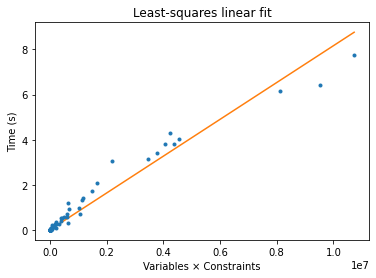
\includegraphics[width=0.9\textwidth]{images/least-squares-solve.png}
\caption{\solve execution time vs. $\norm{V}\norm{C}$ \\ (blue dots), linear model (orange line)}
\label{fig:stats:linregress-solve}
\end{subfigure}
\hfill
\begin{subfigure}{0.475\textwidth}
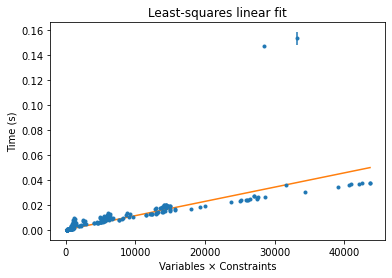
\includegraphics[width=0.9\textwidth]{images/least-squares-RecCheck.png}
\caption{\RecCheck execution time vs. $\norm{V}\norm{C}$ \\ (blue dots), linear model (orange line)}
\label{fig:stats:linregress-reccheck}
\end{subfigure}
\\[3ex]
\begin{subfigure}{0.475\textwidth}
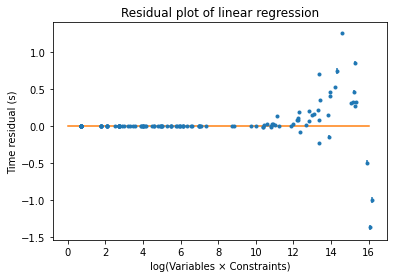
\includegraphics[width=0.9\textwidth]{images/residuals-solve.png}
\caption{\solve model residuals plot (log scale)}
\label{fig:stats:residuals-solve}
\end{subfigure}
\hfill
\begin{subfigure}{0.475\textwidth}
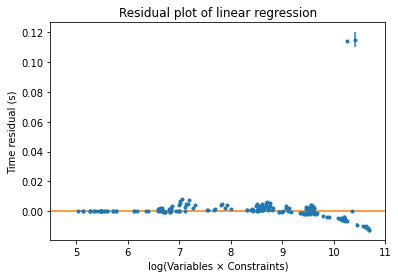
\includegraphics[width=0.9\textwidth]{images/residuals-RecCheck.png}
\caption{\RecCheck model residuals plot (log scale)}
\label{fig:stats:residuals-reccheck}
\end{subfigure}
\\[3ex]
\begin{subfigure}{0.475\textwidth}
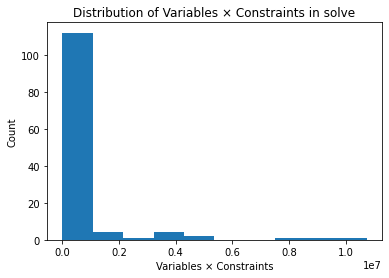
\includegraphics[width=0.9\textwidth]{images/distribution-solve.png}
\caption{$\norm{V}\norm{C}$ distribution in \solve, 10 bins}
\label{fig:stats:distr-solve}
\end{subfigure}
\hfill
\begin{subfigure}{0.475\textwidth}
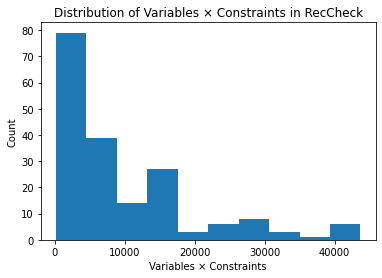
\includegraphics[width=0.9\textwidth]{images/distribution-RecCheck.png}
\caption{$\norm{V}\norm{C}$ distribution in \RecCheck, 10 bins}
\label{fig:stats:distr-reccheck}
\end{subfigure}
\\[2ex]
\caption{Execution vs. $\norm{V}\norm{C}$, residuals, $\norm{V}\norm{C}$ distributions for \solve and \RecCheck}
\label{fig:stats}
\end{figure}

\begin{figure}
\begin{minted}{coq}
Unset Guard Checking.
Set Sized Typing.
Time Definition nats1  := (nat, nat, nat, nat, nat, nat, nat, nat).
Time Definition nats2  := (nats1, nats1, nats1, nats1).
Time Definition nats3  := (nats2, nats2, nats2, nats2).
Time Definition nats4  := (nats3, nats3, nats3, nats3).
Time Definition nats5  := (nats4, nats4, nats4, nats4).
Time Definition nats6  := (nats5, nats5, nats5, nats5).
\end{minted}
\caption{Coq definitions with an explosion in size variables and elapsed time}
\label{fig:nats}
\end{figure}

\subsubsection{Confirming Time Complexity of \solve and \RecCheck}

As shown in \autoref{sec:algorithm}, given a constraint graph from constraint graph $C$ with size variables $V$,
the time complexities of \solve and \RecCheck are $O(\norm{V}\norm{C})$.
Indeed, in \autoref{fig:stats:linregress}, plotting the mean execution times of each of the 301 calls to \solve and 9 calls to \RecCheck
against the number of variables multiplied by the number constraints involved in each call,
we see a strong positive correlation ($r = 0.995$).

To verify that the execution time is dominated by a linear relationship to $\norm{V}\norm{C}$ at large values, we fit the data to a linear model and quantify the goodness of fit.
Using a na\"ive ordinary least-squares regression, the residual plot reveals a fair amount of increase in variability of the residuals roughly proportional to $\norm{V}\norm{C}$ (i.e. the data is heteroskedastic).
This could be explained by the fact that with more variables and constants, the shape of the constraint graph varies more as well.
To take this into account, we instead use a least-squares \emph{percentage} regression~\citep{lspr},
which minimizes the sum of \emph{relative} squared residuals.
The model, overlaid on \autoref{fig:stats:linregress}, is a good fit ($R^2 = 0.999$), with the the resulting relative residuals plot in \autoref{fig:stats:residuals}
(note the logarithmic scale of the independent variable used for clarity).

For large values of $\norm{V}\norm{C}$, the residuals are scattered uniformly about zero, indicating that the linear model is suitable.
For smaller values, the residuals appear to follow some unexplained pattern,
possibly due to dominance of other factors proportional to, say, $\norm{V}$ or $\norm{C}$, due to traversal of the size variable set or constaint set.
\autoref{fig:stats:residuals-zoom} show the absolute residuals at these smaller values;
since they are smaller than half a millesecond, these effects may be due to other irrelevant noise.

\subsubsection{An Explosion of Size Variables}

Now that we have verified the time complexities of \solve and \RecCheck,
we can conclude that the performance degredation is likely due to a large number of variables and constraints involved in these calls.
Although the distribution of $\norm{V}\norm{C}$ in \autoref{fig:stats:vcs-distr} (note again the logarithmic scale) shows that most calls to \solve and \RecCheck involve a small number of variables and constraints,
there are some calls that involve a very large number of them and contribute greatly to the execution time;
the largest takes more than a minute to run.
\autoref{table:large-vcs} lists the nine largest number of variables and constraints in a single call.

\begin{table}
\centering
\begin{tabular}{|r | r | r |}
\hline
\textbf{$\norm{V}$} & \textbf{$\norm{C}$} & \textbf{$\norm{V}\norm{C}$} \\
\hline
%  750 &   592 &    444000 \\
%  908 &   518 &    470344 \\
 1759 &  1417 &   2492503 \\
 3017 &  2261 &   6821437 \\
 3303 &  3071 &  10143513 \\
 4108 &  3619 &  14866852 \\
 4663 &  4282 &  19966966 \\
 4973 &  4159 &  20682707 \\
 6778 &  5184 &  35137152 \\
 7936 &  6641 &  52702976 \\
13197 & 10030 & 132365910 \\
\hline
\end{tabular}
\caption{Largest numbers of variables and constraints involved in individual calls to \solve and \RecCheck}
\label{table:large-vcs}
\end{table}

Although the presence of large numbers of variables and constraints of merely \fieldtheorysized doesn't tell us whether this is a common property of Coq files on average,
the fact that this occurs in the standard library indicates that it is aboslutely possible for an explosion in size variables and constraints to be a significant barrier to the adoption of sized typing for general-purpose use.
In fact, this behaviour is easily reproducible with the artificial but comparatively simple example in \autoref{fig:nateq}.
\autoref{table:large-nateq} lists the number of size variables present in the types and bodies of these definitions,
along with the elapsed type checking time reported by Coq.

\begin{figure}[h]
\begin{minted}{coq}
Unset Guard Checking.
Set Sized Typing.
Time Definition natCst  (n m : nat) := n.
Time Definition natEq1  (n m : nat) : natCst  n m = natCst  n m := eq_refl.
Time Definition natEq2  (n m : nat) : natEq1  n m = natEq1  n m := eq_refl.
Time Definition natEq3  (n m : nat) : natEq2  n m = natEq2  n m := eq_refl.
Time Definition natEq4  (n m : nat) : natEq3  n m = natEq3  n m := eq_refl.
Time Definition natEq5  (n m : nat) : natEq4  n m = natEq4  n m := eq_refl.
Time Definition natEq6  (n m : nat) : natEq5  n m = natEq5  n m := eq_refl.
Time Definition natEq7  (n m : nat) : natEq6  n m = natEq6  n m := eq_refl.
Time Definition natEq8  (n m : nat) : natEq7  n m = natEq7  n m := eq_refl.
Time Definition natEq9  (n m : nat) : natEq8  n m = natEq8  n m := eq_refl.
Time Definition natEq10 (n m : nat) : natEq9  n m = natEq9  n m := eq_refl.
Time Definition natEq11 (n m : nat) : natEq10 n m = natEq10 n m := eq_refl.
Time Definition natEq12 (n m : nat) : natEq11 n m = natEq11 n m := eq_refl.
Time Definition natEq13 (n m : nat) : natEq12 n m = natEq12 n m := eq_refl.
Time Definition natEq14 (n m : nat) : natEq13 n m = natEq13 n m := eq_refl.
Time Definition natEq15 (n m : nat) : natEq14 n m = natEq14 n m := eq_refl.
Time Definition natEq16 (n m : nat) : natEq15 n m = natEq15 n m := eq_refl.
\end{minted}
\caption{Coq definitions with an explosion in size variables and elapsed time}
\label{fig:nateq}
\end{figure}

\begin{table}
\centering
\begin{tabular}{| l | r | r | r | r |}
\hline
\textbf{Definition} & \textbf{$\norm{V}$ (body)} & \textbf{$\norm{V}$ (type)} & \textbf{Total $\norm{V}$} & \textbf{Time (s)} \\
\hline
\coqinline{natCst}  &  0      & 2       & 2       &  0.000 \\
\coqinline{natEq1}  &  1      & 3       & 4       &  0.001 \\
\coqinline{natEq2}  &  2      & 4       & 6       &  0.003 \\
\coqinline{natEq3}  &  4      & 8       & 12      &  0.006 \\
\coqinline{natEq4}  &  11     & 25      & 36      &  0.010 \\
\coqinline{natEq5}  &  33     & 79      & 112     &  0.016 \\
\coqinline{natEq6}  &  94     & 228     & 322     &  0.024 \\
\coqinline{natEq7}  &  252    & 612     & 864     &  0.038 \\
\coqinline{natEq8}  &  647    & 1569    & 2216    &  0.096 \\
\coqinline{natEq9}  &  1617   & 3915    & 5532    &  0.112 \\
\coqinline{natEq10} &  3978   & 9620    & 13598   &  0.179 \\
\coqinline{natEq11} &  9700   & 23440   & 33140   &  0.313 \\
\coqinline{natEq12} &  23539  & 56857   & 80396   &  0.696 \\
\coqinline{natEq13} &  56977  & 137591  & 194568  &  1.626 \\
\coqinline{natEq14} &  137734 & 332564  & 470298  &  4.019 \\
\coqinline{natEq15} &  332732 & 803340  & 1136072 & 10.659 \\
\coqinline{natEq16} &  803535 & 1939969 & 2743504 & 26.112 \\
\hline
\end{tabular}
\caption{Size variables and time elapsed for definitions in \autoref{fig:nateq}}
\label{table:large-nateq}
\end{table}

There are two things we can do to reduce the execution time of \solve and \RecCheck:
eliminate constraints when possible, or reduce the number of size variables in definitions.
One way to accomplish the first option would be to turn on sized typing only for certain definitions,
in particular the ones involving \cofixpoints where they will be most useful.
Then for all other definitions, since no constraints are collected, there will be no calls to \solve,
regardless of how many size variables they contain.

However, a \cofixpoint might require that some non-\corecursive definition with many size variables be size-preserving,
which means that that definition also needs to be checked with sized typing on,
or the \cofixpoint itself may have a large number of size variables.
Furthermore, there's no clear indication of which definitions might have a large number of size variables and which don't,
leaving it up to a lot of guesswork and experimentation.
Using sized typing as a targeted tool for particular programs isn't viable
if we cannot directly tell \emph{which} particular programs will benefit the most
in terms of tradeoffs between non-structural \corecursion and performance.

The second option to reduce the number of size variables can be done by allowing manual annotation of \coinductive types with the infinite size,
reducing the number of free size variables that need to be substituted for
and that propagate throughout subsequent definitions.
For example, the equality types in \autoref{fig:nateq} can have infinite size annotations
without affecting the sizes of either \coqinline{nat} argument.
In other words, we allow size annotations in the surface language that users write,
which would no longer be plain CIC;
as this solution deviates from the philosophy of being wholly backward-compatible,
it is beyond the scope of this paper.

\subsection{Inferring Recursive Indices}\label{sec:impl:recind}

As previously mentioned, users are not obligated to indicate which fixpoint argument is the one on which we recur,
and its position index is inferred during pretyping in the kernel.
In Coq, for a mutual fixpoint, this is done by trying the guard check on every combination of indices%
\footnote{This is the \texttt{search\_guard} function in \texttt{coq/kernel/Pretyping.ml}.}.
This is possible because the guard check is a syntactic check, requiring nothing but the elaborated fixpoint term.

Unfortunately, we run into problems when attempting to apply the same strategy to inferring recursive indices through sized typing alone.
Because termination checking is inextricably tied to type checking,
the entire fixpoint needs to be type checked to verify whether the current set of indices is correct,
and this type checking in the kernel can fail if the fixpoint still contains unsolved metavariables.
Furthermore, because we only have access to the bare environments (\ie with no sizes inferred),
local definitions in scope at the fixpoint may not yet known to be size-preserving,
thus causing the check to fail.
As an example, in the following Coq term, \coqinline{id} has no size annotations and is therefore treated as \emph{not} size-preserving,
even though it ought to be, which causes the recursive call on the smaller argument wrapped in \coqinline{id} to not pass type checking.

\begin{minted}{coq}
let id (x : nat) := x in
  fix f (n : nat) :=
    match n with
    | O => O
    | S k => f (id k)
    end
\end{minted}

This suggests that size inference should be done during the pretyping phase:
size inference could be viewed as part of the elaboration step from the surface CIC to the core \lang.
This, too, is beyond the scope of this paper, especially as there is no past work on the interaction between size inference and elaboration to build on.
